%----------------------------------------------------  
  \vspace{0.3cm}
  
  \tex\section{Introdução}
\begin{frame}{Introdução}
  \textbf{Porquê é importante}: As baterias alimentam veícul\begin{frame}{Abordagem Selecionada: \begin{frame}{Metodologia}
  \begin{block}{Ad\section{Experiências}
\begin{frame}{Experiências: Conjunto de Dados}
  \begin{block}{\begin{frame}{Resultados: Visualizações}
  \begin{itemize}
    \item \textbf{Previsão SOC}: Aco\begin{frame}[plain]
  \cent% Bibliography
\begin{frame}{Referências}
  \begin{thebibliography}{9}
    \bibitem{timesnet}
      Haixu Wu, Tengge Hu, Yong Liu, Hang Zhou, Jianmin Wang, Mingsheng Long.
      \emph{TimesNet: Temporal 2D-Variation Modeling for General Time Series Analysis}.
      ICLR, 2023.
    
    \bibitem{calce}
      CALCE Battery Research Group.
      \emph{Lithium-ion Battery Experimental Data}.
      University of Maryland.
      
    \bibitem{optuna}
      Takuya Akiba, Shotaro Sano, Tetsuya Teshima, Takeru Ohta, Masanori Koyama.
      \emph{Optuna: A Next-generation Hyperparameter Optimization Framework}.
      KDD, 2019.
  \end{thebibliography}
\end{frame}bf{Obrigado!}
  
  \vspace{1cm}
  
  \normalsize
  Perguntas?
  
  \vspace{0.5cm}
  \small
  Pedro André Silva Ferreira
  Julho 2025
\end{frame}o os valores reais
    \item \textbf{SOH/RUL}: Precisão moderada, margem para melhoria
  \end{itemize}
  
  \vspace{0.5cm}
  
  \centering
  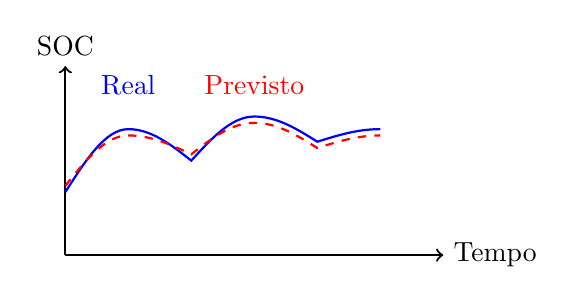
\begin{tikzpicture}[scale=0.8]
    % Prediction vs actual visualization
    \draw[thick, ->] (0,0) -- (6,0) node[right] {Tempo};
    \draw[thick, ->] (0,0) -- (0,3) node[above] {SOC};
    
    \draw[blue, thick] (0,1) sin (1,2) cos (2,1.5) sin (3,2.2) cos (4,1.8) sin (5,2);
    \draw[red, dashed, thick] (0,1.1) sin (1,1.9) cos (2,1.6) sin (3,2.1) cos (4,1.7) sin (5,1.9);
    
    \node[blue] at (1,2.7) {Real};
    \node[red] at (3,2.7) {Previsto};
  \end{tikzpicture}LCE CS2}
    \begin{itemize}
      \item 886 ciclos de dados de baterias
      \item Pré-processado para cálculos de SOC, SOH, RUL
      \item \textbf{Características Chave}: Tensão, corrente, tendências de capacidade
    \end{itemize}
  \end{block}    \begin{itemize}
      \item \textbf{Entradas}: Tensão, corrente, temperatura, etc.
      \item \textbf{Alvos}: SOC, SOH, RUL
    \end{itemize}
  \end{block}
  
  \vspace{0.3cm}
  
  \textbf{Ferramentas Utilizadas}:
  \begin{itemize}
    \item Otimização de hiperparâmetros com \textbf{Optuna}
    \item Acompanhamento de experiências com \textbf{Weights \& Biases}
  \end{itemize}gin{block}{O que é o TimesNet?}
    \begin{itemize}
      \item Estado da arte para previsão de séries temporais
      \item Usa Transformada Rápida de Fourier (FFT) para detetar períodos
      \item Converte dados 1D em tensores 2D para análise CNN 2D
    \end{itemize}
  \end{block}
  
  \begin{exampleblock}{Porquê se adequa}
    Captura padrões de bateria de curto e longo prazo eficazmente
  \end{exampleblock} e comboios, sendo críticas para a segurança e eficiência.
  
  \vspace{0.5cm}
  
  \begin{block}{Objetivo: Usar IA para prever}
    \begin{itemize}
      \item \textbf{Estado de Carga (SOC)}: Nível de energia atual
      \item \textbf{Estado de Saúde (SOH)}: Condição da bateria
      \item \textbf{Vida Útil Remanescente (RUL)}: Tempo até substituição
    \end{itemize}
  \end{block}das Baterias}:
  \begin{itemize}
    \item \textbf{Ião-lítio (Li-ion)}: Alta densidade energética, longa vida, usado em veículos elétricos/comboios
    \item \textbf{Chumbo-ácido}: Pesado, baixa energia, usado em veículos tradicionais
    \item \textbf{Níquel-hidreto metálico (NiMH)}: Veículos híbridos, menos energia que Li-ion
    \item \textbf{Estado sólido}: Emergente, maior densidade, mais seguro, ainda em desenvolvimento
  \end{itemize}
  
  \begin{exampleblock}{Porquê Li-ion?}
    Ideal para transporte devido à eficiência e fiabilidade.
  \end{exampleblock}----------------------
%    PACKAGES AND THEMES
%----------------------------------------------------------------------------------------
\documentclass[aspectratio=169,xcolor=dvipsnames]{beamer}
\makeatletter
\def\input@path{{theme/}}
\makeatother
\usetheme{CleanEasy}
\usepackage[utf8]{inputenc}
\usepackage{lmodern}
\usepackage[T1]{fontenc}
\usepackage[portuguese]{babel}
\usepackage{fix-cm}
\usepackage{amsmath}
\usepackage{mathtools}
\usepackage{listings}
\usepackage{xcolor}
\usepackage{hyperref}
\usepackage{graphicx} % Allows including images
\usepackage{booktabs} % Allows the use of \toprule, \midrule and \bottomrule in tables
\usepackage{tikz}
\usetikzlibrary{positioning, shapes, arrows, calc, decorations.pathreplacing, arrows.meta, backgrounds, patterns, overlay-beamer-styles}
\usepackage{etoolbox}
\usepackage{animate}

%----------------------------------------------------------------------------------------
%    LAYOUT CONFIGURATION
%----------------------------------------------------------------------------------------
\input{configs/configs}
%----------------------------------------------------------------------------------------
%    TITLE PAGE
%----------------------------------------------------------------------------------------
%---------------------------------------------


\title[BattAIHealth]{BattAIHealth: AI for Battery Health Monitoring}

\author[Pedro Ferreira]{Pedro André Silva Ferreira}

\institute{Engenharia Eletrotécnica e de Computadores\\Ramo de Eletrónica e Computadores }

\date{21 Julho 2025}
% Define positions for logos on title page
\titlegraphic{
  \begin{tikzpicture}[remember picture, overlay]
    % ESTG Logo
    \node[anchor=north east, xshift=-0.8cm, yshift=-0.3cm] at (current page.north east) {
      \includegraphics[height=1.5cm]{logos/estg_h.pdf}
    };
  \end{tikzpicture}
}


%----------------------------------------------------------------------------------------


\begin{document}

\begin{frame}[plain]
  \titlepage
\end{frame}

\begin{frame}[plain]{Conteúdos}
  \tableofcontents
\end{frame}

\section{Fundamentos das Baterias}
\begin{frame}{Fundamentos das Baterias: Introdução às Químicas}
  \begin{block}{O que é uma bateria?}
    Um dispositivo eletroquímico que armazena e liberta energia através de reações químicas.
  \end{block}
  
  \textbf{Porque as baterias são importantes}: Alimentam veículos elétricos e comboios, sendo críticas para o transporte moderno.
  
  \vspace{0.3cm}
  
  \textbf{Battery Chemistries}:
  \begin{itemize}
    \item \textbf{Lithium-ion (Li-ion)}: High energy density, long life, used in EVs/trains
    \item \textbf{Lead-acid}: Heavy, low energy, used in traditional vehicles
    \item \textbf{Nickel-metal hydride (NiMH)}: Hybrid vehicles, less energy than Li-ion
    \item \textbf{Solid-state}: Emerging, higher density, safer, still in development
  \end{itemize}
  
  \begin{exampleblock}{Why Li-ion?}
    Ideal for transportation due to efficiency and reliability.
  \end{exampleblock}
\end{frame}

\section{Introduction}
\begin{frame}{Introduction}
  \textbf{Why it matters}: Batteries power EVs and trains, critical for safety and efficiency.
  
  \vspace{0.5cm}
  
  \begin{block}{Goal: Use AI to predict}
    \begin{itemize}
      \item \textbf{State of Charge (SOC)}: Current energy level
      \item \textbf{State of Health (SOH)}: Battery condition
      \item \textbf{Remaining Useful Life (RUL)}: Time until replacement
    \end{itemize}
  \end{block}
  
  \vspace{0.5cm}
  
  \centering
  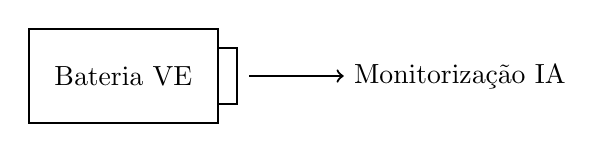
\begin{tikzpicture}[scale=0.8]
    % Simple battery illustration
    \draw[thick] (0,0) rectangle (3,1.5);
    \draw[thick] (3,0.3) rectangle (3.3,1.2);
    
    \node at (1.5,0.75) {Bateria VE};
    \draw[thick, ->] (3.5,0.75) -- (5,0.75) node[right] {Monitorização IA};
  \end{tikzpicture}
\end{frame}

\section{Métodos}
\begin{frame}{Estado da Arte}
  \begin{columns}
    \begin{column}{0.48	extwidth}
      	extbf{Métodos Tradicionais}:
      \begin{itemize}
        \item Filtros de Kalman
        \item Modelos de circuito equivalente
      \end{itemize}
      
      \begin{alertblock}{Limitações}
        Dificuldades com não-linearidade e variabilidade
      \end{alertblock}
    \end{column}
    \begin{column}{0.48	extwidth}
      	extbf{Vantagem da IA}:
      \begin{itemize}
        \item Aprendizagem profunda captura padrões complexos dos dados
      \end{itemize}
      
      \begin{exampleblock}{Benefícios}
        Melhor tratamento de relações complexas e não-lineares
      \end{exampleblock}
    \end{column}
  \end{columns}
  
  \vspace{0.5cm}
  
  \centering
  
\begin{tikzpicture}[scale=0.7]
    % Traditional vs AI comparison
    \draw[thick] (0,0) rectangle (2,1) node[pos=.5] {Tradicionais};
    \draw[thick] (3,0) rectangle (5,1) node[pos=.5] {Métodos IA};
    \draw[thick, ->] (2.2,0.5) -- (2.8,0.5);
  \end{tikzpicture}
\end{frame}

\begin{frame}{Métodos Base}
  \textbf{Métodos Explorados}:
  
  \begin{itemize}
    \item \textbf{Transformer}: Alta precisão, computacionalmente pesado
    \item \textbf{Mistura de Especialistas (MoE)}: Eficiente, resultados competitivos
  \end{itemize}
  
  \vspace{0.5cm}
  
  \begin{block}{Método Escolhido: TimesNet}
    Excele em padrões multi-periódicos em dados de baterias
  \end{block}
  
  \vspace{0.5cm}
  
  \begin{table}
    \centering
    \caption{Comparação de Desempenho}
    \begin{tabular}{lc}
      \toprule
      \textbf{Método} & \textbf{Desempenho} \\
      \midrule
      Transformer & Alto \\
      MoE & Competitivo \\
      TimesNet & \textbf{Melhor} \\
      \bottomrule
    \end{tabular}
  \end{table}
\end{frame}

\begin{frame}{Selected Approach: TimesNet}
  \begin{block}{What is TimesNet?}
    \begin{itemize}
      \item State-of-the-art for time series forecasting
      \item Uses Fast Fourier Transform (FFT) to detect periods
      \item Converts 1D data to 2D tensors for 2D CNN analysis
    \end{itemize}
  \end{block}
  
  \begin{exampleblock}{Why it fits}
    Captures short- and long-term battery patterns effectively
  \end{exampleblock}
  
  \vspace{0.5cm}
  
  \centering
  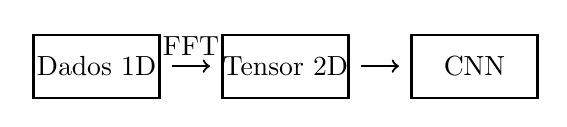
\begin{tikzpicture}[scale=0.8]
    % TimesNet architecture visualization
    \draw[thick] (0,0) rectangle (2,1) node[pos=.5] {Dados 1D};
    \draw[thick, ->] (2.2,0.5) -- (2.8,0.5) node[midway,above] {FFT};
    \draw[thick] (3,0) rectangle (5,1) node[pos=.5] {Tensor 2D};
    \draw[thick, ->] (5.2,0.5) -- (5.8,0.5);
    \draw[thick] (6,0) rectangle (8,1) node[pos=.5] {CNN};
  \end{tikzpicture}
\end{frame}

\begin{frame}{Methodology}
  \begin{block}{Adaptation}
    \begin{itemize}
      \item \textbf{Inputs}: Voltage, current, temperature, etc.
      \item \textbf{Targets}: SOC, SOH, RUL
    \end{itemize}
  \end{block}
  
  \vspace{0.3cm}
  
  \textbf{Tools Used}:
  \begin{itemize}
    \item Hyperparameter tuning with \textbf{Optuna}
    \item Experiment tracking with \textbf{Weights \& Biases}
  \end{itemize}
  
  \vspace{0.5cm}
  
  \centering
  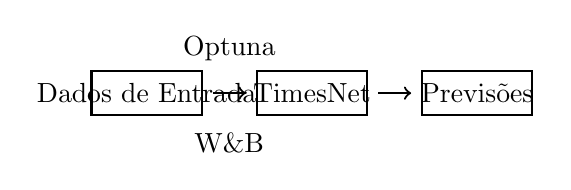
\begin{tikzpicture}[scale=0.7]
    % Methodology flowchart
    \draw[thick] (0,0) rectangle (2,0.8) node[pos=.5] {Dados de Entrada};
    \draw[thick, ->] (2.2,0.4) -- (2.8,0.4);
    \draw[thick] (3,0) rectangle (5,0.8) node[pos=.5] {TimesNet};
    \draw[thick, ->] (5.2,0.4) -- (5.8,0.4);
    \draw[thick] (6,0) rectangle (8,0.8) node[pos=.5] {Previsões};
    
    \node at (2.5,1.2) {Optuna};
    \node at (2.5,-0.5) {W\&B};
  \end{tikzpicture}
\end{frame}

\section{Experiments}
\begin{frame}{Experiments: Dataset}
  \begin{block}{CALCE CS2 Dataset}
    \begin{itemize}
      \item 886 cycles of battery data
      \item Preprocessed for SOC, SOH, RUL calculations
      \item \textbf{Key Features}: Voltage, current, capacity trends
    \end{itemize}
  \end{block}
  
  \vspace{0.5cm}
  
  \centering
  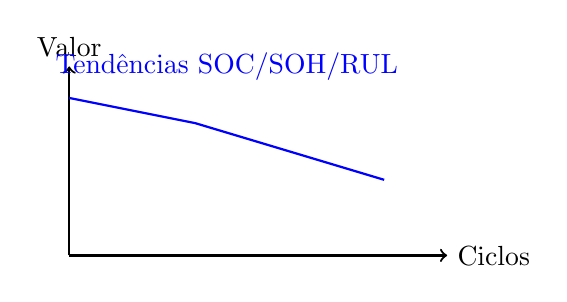
\begin{tikzpicture}[scale=0.8]
    % Data visualization concept
    \draw[thick, ->] (0,0) -- (6,0) node[right] {Ciclos};
    \draw[thick, ->] (0,0) -- (0,3) node[above] {Valor};
    
    \draw[blue, thick] (0,2.5) -- (1,2.3) -- (2,2.1) -- (3,1.8) -- (4,1.5) -- (5,1.2);
    
    \node[blue] at (2.5,3) {Tendências SOC/SOH/RUL};
  \end{tikzpicture}
\end{frame}

\begin{frame}{Experiências: Treino}
  \begin{block}{Configuração de Treino}
    \begin{itemize}
      \item 43 épocas, 30,81 horas de tempo de treino
      \item Perda de validação final: 0,02929
      \item Otimizado com Optuna (50 tentativas)
      \item Monitorizado via Weights \& Biases
    \end{itemize}
  \end{block}
  
  \vspace{0.5cm}
  
  \centering
  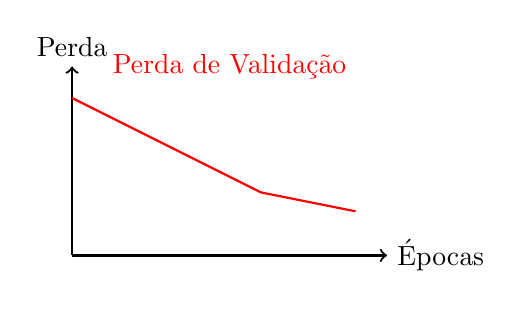
\begin{tikzpicture}[scale=0.8]
    % Training curve visualization
    \draw[thick, ->] (0,0) -- (5,0) node[right] {Épocas};
    \draw[thick, ->] (0,0) -- (0,3) node[above] {Perda};
    
    \draw[red, thick] (0,2.5) .. controls (1,2) and (2,1.5) .. (3,1) .. controls (4,0.8) .. (4.5,0.7);
    
    \node[red] at (2.5,3) {Perda de Validação};
  \end{tikzpicture}
\end{frame}

\section{Resultados}
\begin{frame}{Resultados: Métricas de Desempenho}
  \begin{block}{Métricas de Desempenho (RMSE)}
    \begin{itemize}
      \item \textbf{SOC}: 0,2251 (melhor desempenho)
      \item \textbf{SOH}: 0,5252
      \item \textbf{RUL}: 0,5311 (mais desafiador)
    \end{itemize}
  \end{block}
  
  \begin{exampleblock}{Perspetiva}
    SOC é mais fácil de prever, RUL é mais difícil devido à complexidade de previsão a longo prazo
  \end{exampleblock}
  
  \vspace{0.5cm}
  
  \begin{table}
    \centering
    \caption{Valores RMSE por Alvo}
    \begin{tabular}{lc}
      \toprule
      \textbf{Alvo} & \textbf{RMSE} \\
      \midrule
      SOC & 0,2251 \\
      SOH & 0,5252 \\
      RUL & 0,5311 \\
      \bottomrule
    \end{tabular}
  \end{table}
\end{frame}

\begin{frame}{Results: Visualizations}
  \begin{itemize}
    \item \textbf{SOC Prediction}: Closely tracks actual values
    \item \textbf{SOH/RUL}: Moderate accuracy, room for improvement
  \end{itemize}
  
  \vspace{0.5cm}
  
  \centering
  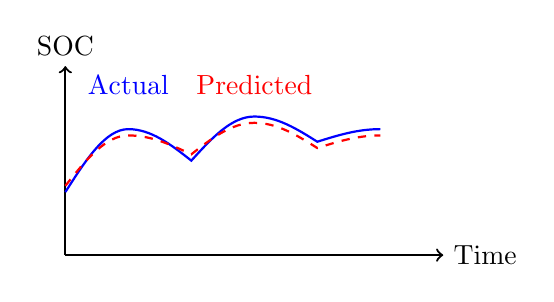
\begin{tikzpicture}[scale=0.8]
    % Prediction vs actual visualization
    \draw[thick, ->] (0,0) -- (6,0) node[right] {Time};
    \draw[thick, ->] (0,0) -- (0,3) node[above] {SOC};
    
    \draw[blue, thick] (0,1) sin (1,2) cos (2,1.5) sin (3,2.2) cos (4,1.8) sin (5,2);
    \draw[red, dashed, thick] (0,1.1) sin (1,1.9) cos (2,1.6) sin (3,2.1) cos (4,1.7) sin (5,1.9);
    
    \node[blue] at (1,2.7) {Actual};
    \node[red] at (3,2.7) {Predicted};
  \end{tikzpicture}
\end{frame}

\section{Discussão}
\begin{frame}{Discussão}
  \begin{alertblock}{Desafios}
    \begin{itemize}
      \item Aprendizagem multi-tarefa dilui desempenho vs. modelos especializados
      \item Compromisso: Modelo unificado vs. precisão específica da tarefa
      \item Alta complexidade limita implementação em tempo real
    \end{itemize}
  \end{alertblock}
  
  \vspace{0.5cm}
  
  \centering
  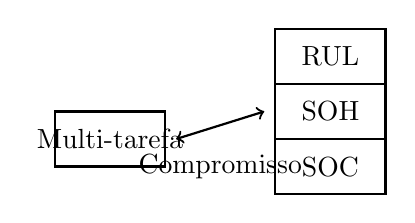
\begin{tikzpicture}[scale=0.7]
    % Multi-task trade-off diagram
    \draw[thick] (0,1) rectangle (2,2) node[pos=.5] {Multi-tarefa};
    \draw[thick] (4,0.5) rectangle (6,1.5) node[pos=.5] {SOC};
    \draw[thick] (4,1.5) rectangle (6,2.5) node[pos=.5] {SOH};
    \draw[thick] (4,2.5) rectangle (6,3.5) node[pos=.5] {RUL};
    
    \draw[thick, <->] (2.2,1.5) -- (3.8,2);
    \node at (3,1) {Compromisso};
  \end{tikzpicture}
\end{frame}

\section{Conclusão}
\begin{frame}{Conclusão \& Trabalho Futuro}
  \begin{block}{Conquistas}
    \begin{itemize}
      \item Adaptação bem-sucedida do TimesNet para monitorização da saúde de baterias
      \item Obtidos conhecimentos sobre limitações da aprendizagem multi-tarefa
      \item Demonstrado potencial da IA em aplicações de baterias
    \end{itemize}
  \end{block}
  
  \begin{exampleblock}{Direções Futuras}
    \begin{itemize}
      \item Desenvolver modelos especializados por tarefa
      \item Explorar modelos híbridos IA-físicos
      \item Criar designs eficientes para implementação em tempo real
    \end{itemize}
  \end{exampleblock}
  
  \vspace{0.5cm}
  
  \centering
  
\begin{tikzpicture}[scale=0.6]
    % Future work icons
    \draw[thick] (0,0) circle (0.5) node {IA};
    \draw[thick] (2,0) circle (0.5) node {Tempo Real};
    \draw[thick] (4,0) circle (0.5) node {Híbrido};
    \end{tikzpicture}
\end{frame}

\begin{frame}[plain]
  \centering
  \Huge \textbf{Thank you!}
  
  \vspace{1cm}
  
  \normalsize
  Questions?
  
  \vspace{0.5cm}
  \small
  Pedro André Silva Ferreira
  July 2025
\end{frame}

% Bibliography
\begin{frame}{References}
  \begin{thebibliography}{9}
    \bibitem{timesnet}
      Haixu Wu, Tengge Hu, Yong Liu, Hang Zhou, Jianmin Wang, Mingsheng Long.
      \emph{TimesNet: Temporal 2D-Variation Modeling for General Time Series Analysis}.
      ICLR, 2023.
    
    \bibitem{calce}
      CALCE Battery Research Group.
      \emph{Lithium-ion Battery Experimental Data}.
      University of Maryland.
      
    \bibitem{optuna}
      Takuya Akiba, Shotaro Sano, Tetsuya Teshima, Takeru Ohta, Masanori Koyama.
      \emph{Optuna: A Next-generation Hyperparameter Optimization Framework}.
      KDD, 2019.
  \end{thebibliography}
\end{frame}

\end{document}

\section{Methods}
\begin{frame}{Lists and Numbering}
  \begin{columns}
    \begin{column}{0.48\textwidth}
      Bulleted list:
      \begin{itemize}
        \item First level item
        \begin{itemize}
          \item Second level item
          \item Another second level
          \begin{itemize}
            \item Third level item
          \end{itemize}
        \end{itemize}
        \item Another first level item
      \end{itemize}
    \end{column}
    \begin{column}{0.48\textwidth}
      Numbered list:
      \begin{enumerate}
        \item First step
        \begin{enumerate}
          \item Substep one
          \item Substep two
        \end{enumerate}
        \item Second step
        \item Third step
      \end{enumerate}
    \end{column}
  \end{columns}
\end{frame}

\begin{frame}{Tables}
  \begin{table}
    \centering
    \caption{Sample table with booktabs style}
    \begin{tabular}{lcr}
      \toprule
      \textbf{Header 1} & \textbf{Header 2} & \textbf{Header 3} \\
      \midrule
      Row 1, Col 1 & Row 1, Col 2 & 123.45 \\
      Row 2, Col 1 & Row 2, Col 2 & 67.89 \\
      Row 3, Col 1 & Row 3, Col 2 & 456.78 \\
      \bottomrule
    \end{tabular}
  \end{table}
  
  \vspace{0.5cm}
  
  \begin{block}{Table styling}
    The CleanEasy theme works well with the booktabs package for professional-looking tables. 
    Simple color alterations make tables more readable without being distracting.
  \end{block}
\end{frame}

\begin{frame}{Mathematical Equations}
  The CleanEasy theme includes proper mathematical typesetting:
  
  \begin{align}
    E &= mc^2 \\
    F &= G\frac{m_1 m_2}{r^2}
  \end{align}
  
  Maxwell's equations in differential form:
  \begin{align}
    \nabla \cdot \vec{E} &= \frac{\rho}{\varepsilon_0} \\
    \nabla \cdot \vec{B} &= 0 \\
    \nabla \times \vec{E} &= -\frac{\partial \vec{B}}{\partial t} \\
    \nabla \times \vec{B} &= \mu_0 \vec{J} + \mu_0\varepsilon_0\frac{\partial \vec{E}}{\partial t}
  \end{align}
  
  Inline equations like $E = mc^2$ are also properly rendered.
\end{frame}

\begin{frame}[fragile]{Code Listings}
  \begin{lstlisting}[language=Python]
# A simple Python function
def fibonacci(n):
    """Return the nth Fibonacci number"""
    if n <= 0:
        return 0
    elif n == 1:
        return 1
    else:
        a, b = 0, 1
        for _ in range(2, n + 1):
            a, b = b, a + b
        return b
  
# Calculate the 10th Fibonacci number
result = fibonacci(10)
print(f"The 10th Fibonacci number is {result}")
  \end{lstlisting}
\end{frame}

\begin{frame}{Figures and Graphics}
  \begin{columns}
    \begin{column}{0.48\textwidth}
      \centering
      \begin{figure}
        \centering
        % Replace with actual image path
        % \includegraphics[width=\textwidth]{figures/sample_image.png}
        \tikz \fill[blue!30] (0,0) rectangle (3,2);
        \caption{Sample placeholder image}
      \end{figure}
    \end{column}
    \begin{column}{0.48\textwidth}
      \centering
      \begin{figure}          
      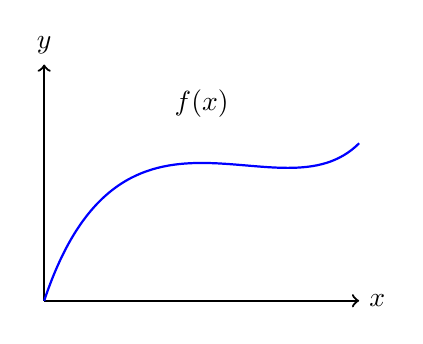
\begin{tikzpicture}
        % Simple TikZ diagram
        \draw[thick, ->] (0,0) -- (4,0) node[right] {$x$};
        \draw[thick, ->] (0,0) -- (0,3) node[above] {$y$};
        \draw[blue, thick] (0,0) .. controls (1,3) and (3,1) .. (4,2);
        \node at (2,2.5) {$f(x)$};
      \end{tikzpicture}
      \caption{Simple TikZ diagram}
       \label{fig:enter-label}
      \end{figure}
    \end{column}
  \end{columns}
\end{frame}

\section{Results}
\begin{frame}{Overlays and Animations}
  Beamer supports step-by-step revelations:
  
  \begin{itemize}
    \item<1-> First point appears on slide 1
    \item<2-> Second point appears on slide 2
    \item<3-> Third point appears on slide 3
  \end{itemize}
  
  \pause
  
  This text appears after a pause.
  
  \onslide<4->{
    And this content appears on slide 4.
  }
  
  \begin{block}<5->{Delayed Block}
    This entire block appears only on slide 5.
  \end{block}
\end{frame}

\begin{frame}{Citations and References}
  CleanEasy works well with bibliographies and citations:
  
  \begin{block}{Sample citation}
    According to Einstein \cite{einstein1905}, space and time are relative.
  \end{block}
  
  \begin{exampleblock}{Bibliography management}
    The theme is compatible with BibTeX, BibLaTeX, and other bibliography management tools.
  \end{exampleblock}
  
  % Sample bibliography entries (not functional without .bib file)
  % \begin{thebibliography}{9}
  % \bibitem{einstein1905}
  %   Albert Einstein.
  %   \emph{On the Electrodynamics of Moving Bodies}.
  %   Annalen der Physik, 1905.
  % \end{thebibliography}
\end{frame}

\begin{frame}{Custom TikZ Graphics}

  \begin{figure}
      \centering
      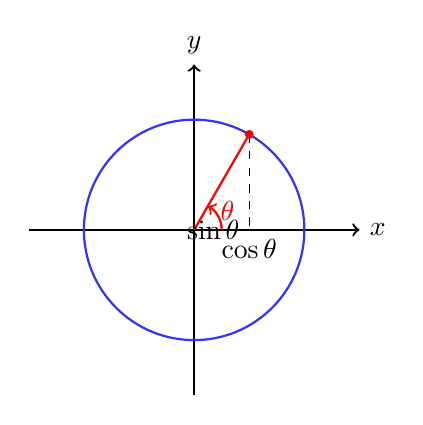
\begin{tikzpicture}[scale=0.7]
        % Coordinate axes
        \draw[thick, ->] (-3,0) -- (3,0) node[right] {$x$};
        \draw[thick, ->] (0,-3) -- (0,3) node[above] {$y$};
        
        % Unit circle
        \draw[blue!80, thick] (0,0) circle (2);
        
        % Angle and point on circle
        \filldraw[red] (60:2) circle (2pt);
        \draw[red, thick] (0,0) -- (60:2);
        \draw[red, thick, ->] (0.5,0) arc (0:60:0.5);
        \node[red] at (30:0.7) {$\theta$};
        
        % Coordinates
        \draw[dashed] (60:2) -- (60:2 |- 0,0) node[below] {$\cos\theta$};
        \draw[dashed] (60:2) -- (0,0 -| 60:2) node[left] {$\sin\theta$};
      \end{tikzpicture}
      \caption{The unit circle with trigonometric functions}
      \label{fig:exampleTikz}
  \end{figure}
\end{frame}

\section{Conclusions}
\begin{frame}{Theme Customization}
  The CleanEasy theme can be easily customized:
  
  \begin{itemize}
    \item Edit \texttt{beamercolorthemeCleanEasy.sty} to change colors
    \item Modify \texttt{beamerfontthemeCleanEasy.sty} for different fonts
    \item Adjust \texttt{beamerinnerthemeCleanEasy.sty} for layout changes
    \item Update \texttt{configs.tex} for footer and section page customization
  \end{itemize}
  
  \begin{alertblock}{Important Note}
    Always maintain consistent design elements throughout your presentation for a professional look.
  \end{alertblock}
\end{frame}

\begin{frame}{Final Thoughts}
  \begin{block}{Benefits of CleanEasy}
    \begin{itemize}
      \item Professional appearance suitable for academic and business contexts
      \item Careful attention to typography and spacing
      \item High readability with suitable contrast ratios
      \item Flexible design that works with different content types
    \end{itemize}
  \end{block}
  
  \vspace{0.5cm}
  
  \begin{center}
    \large{The CleanEasy theme is designed to let your content shine without distractions}
  \end{center}
\end{frame}

\begin{frame}[plain]
  \centering
  \Huge \textbf{Thank you!}
  
  \vspace{1cm}
  \normalsize
  \href{mailto:your@email.com}{your@email.com}
  
  \vspace{0.5cm}
  \small
  \texttt{https://someurl.com}
\end{frame}

% Sample bibliography (not shown in presentation, just for reference)
\begin{frame}{References}
  \begin{thebibliography}{9}
    \bibitem{einstein1905}
      Albert Einstein.
      \emph{On the Electrodynamics of Moving Bodies}.
      Annalen der Physik, 1905.
    
    \bibitem{beamer}
      Till Tantau.
      \emph{The Beamer Class}.
      \url{https://ctan.org/pkg/beamer}
  \end{thebibliography}
\end{frame}

% \begin{frame}{References}
%   \bibliography{reference.bib}
%   \bibliographystyle{apalike}
% \end{frame}

\end{document}